\section{Objective}
To determine the coefficient of thermal expansion ($\alpha$) for a brass rod using Fizeau's
interferometer.

\section{Theory}
Consider a metal bar of length $L$ and $\alpha(T)$ be its coefficient
of thermal expansion. Then the rate of change of its length
with respect to temperature is,
\begin{align}
    \frac{dL}{dT}=\alpha(T)L
\end{align}

For small changes in temperature, we can see that $\alpha(T)$ remains almost a constant and we can make an approximation
\begin{align}
\frac{\Delta L}{\Delta T} \approx \alpha L
\end{align}
From the above expression, we can deduce the working formula
\begin{align}
    \alpha = \frac{1}{L}\left(\frac{\Delta L}{\Delta T}\right)
\end{align}
In order to determine $\alpha$, we need to have changes in length of
rod for different temperature changes. But this length changes
are of the order of 10$^{-3}$, which is not easily measurable. This
problem can be tackled by employing \textbf{Fizeau's method}.

In this method, we have two glass plates fixed together at one
end and placed one (long plate) above the other (short plate).
the non-fixed side of the long plate is allowed to rest on an
insulator, which rests on the expanding rod. So the expansion
of the rod will cause the upper glass plate to rise, creating a
wedge shaped air film between the glass plates. The air film
is then illuminated by a monochromatic light source of wavelength $\lambda$ at normal incidence. Light rays reflected from the
upper and lower glass plates will have a path difference (as
shown in Fig. \ref{fig:1}) and they interfere to produce a fringe pattern
consisting of hyperbolic lines.The instrument that we would
use to carry out the above experiment is Fizeau's interferometer --- which consists of a monochromatic source, a glass that
reflects the light rays towards the inclined glass plates, a holder
for the metal bar and a travelling microscope to see the fringe
pattern and measure fringe width.

\begin{figure}[H]
    \centering
    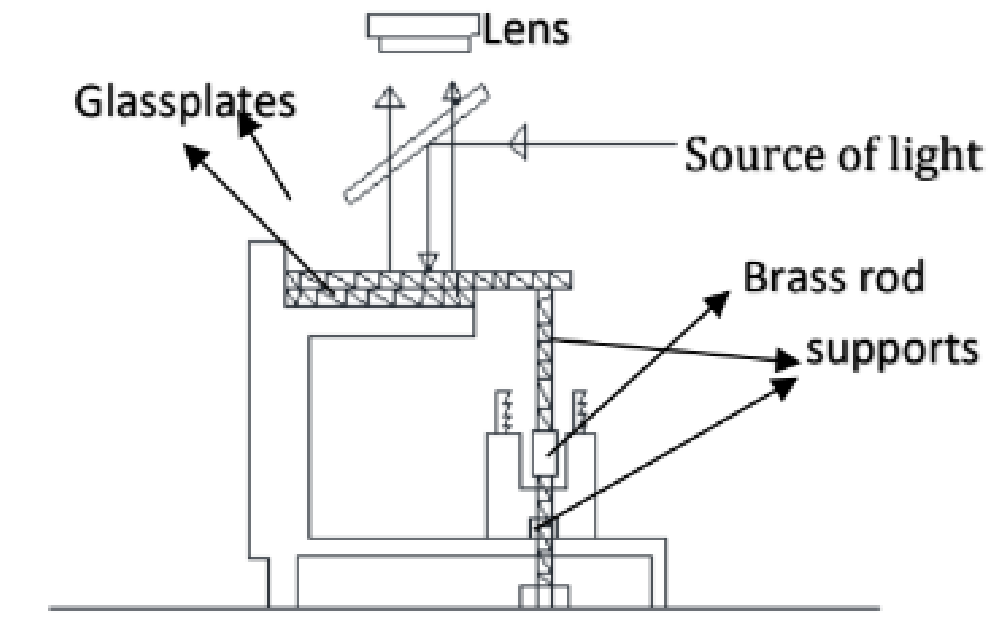
\includegraphics[width=0.8\columnwidth]{images/f1.png}
    \caption{Experimental Setup}
    \label{fig:1}
\end{figure}

Let $t$ be the thickness of the air film between the plates at
some point. The optical path difference between the direct
and reflected rays at that point would be,

\begin{align}
    \Delta = 2t + \frac{\lambda}{2}
\end{align}

For minima, we have

\begin{align}
    \Delta &= (2n+1) \frac{\lambda}{2},\,\,\,n=0, 1, 2, ... \nonumber\\
    \implies 2t + \frac{\lambda}{2} &= (2n+1) \frac{\lambda}{2} \nonumber\\
    \text{or, } t &= \frac{n\lambda}{2}
\end{align}

Now, consider two consecutive dark fringes - let $t_1$ and $t_2$ be
the thickness of the air film at the points where dark fringes
are formed. This is shown in Fig (\ref{fig:2}).

\begin{figure}[H]
    \centering
    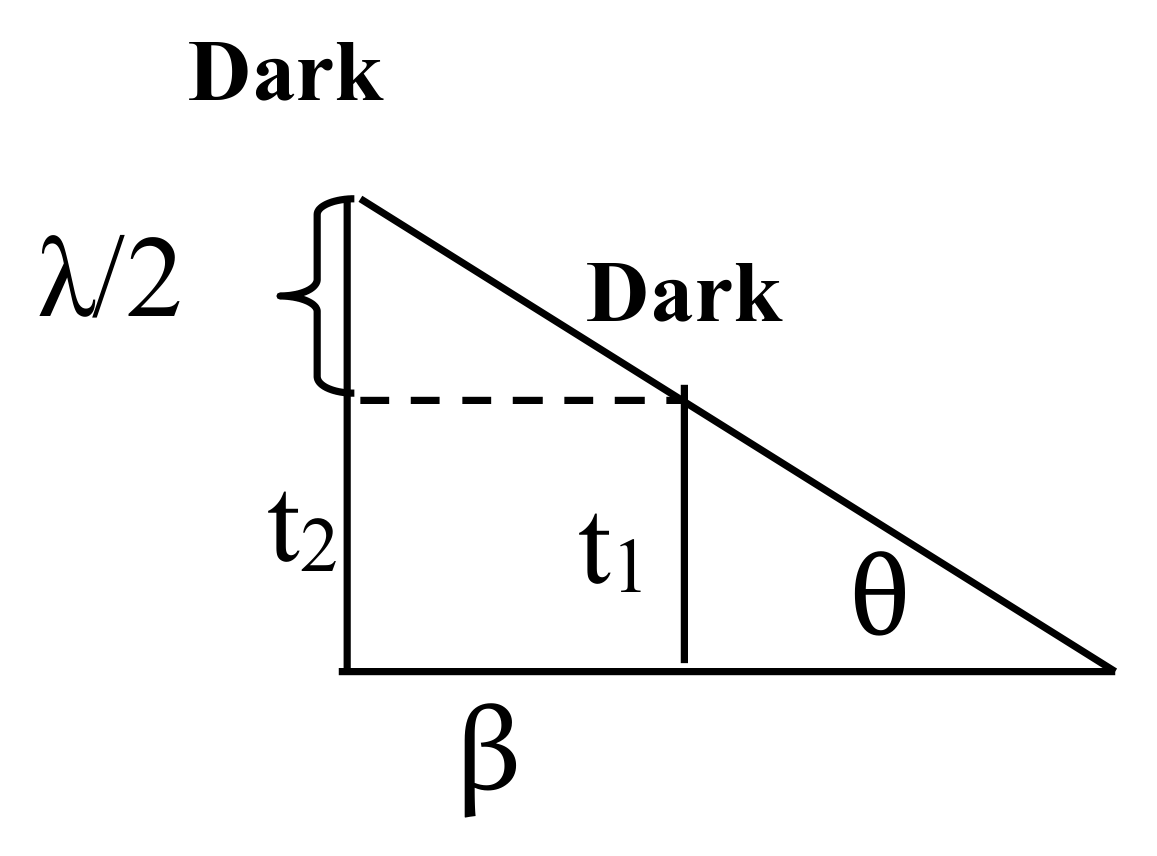
\includegraphics[width=0.5\columnwidth]{images/f2.png}
    \caption{Figure showing the points where two consecu-
    tive dark fringes are formed.}
    \label{fig:2}
\end{figure}

\begin{align}
    t_1 &= m\frac{\lambda}{2} \nonumber \\
    t_2 &= (m+1)\frac{\lambda}{2} \nonumber \\
    \implies t_2 - t_1 &= \frac{\lambda}{2}
\end{align}

From the triangle shown in Fig. (\ref{fig:2}),
\begin{align}
    \tan \theta = \frac{t_2 - t_1}{\beta} = \frac{\lambda}{2\beta}
\end{align}

where, $\beta$ is the fringe width, i.e, the distance between two consecutive minima or maxima.

As the temperature of the metal bar increases, it expands and
pushes up the top glass plate, increasing the wedge angle. Let
$\theta_1$, $\theta_2$ and $\beta_1$, $\beta_2$ be the respective wedge angles and fringe
widths at temperatures $T_1$ and $T_2$. Then,

\begin{align*}
    \tan \theta_1 = \frac{\lambda}{2\beta_1} \implies \theta_1 = \taninv{\left(\frac{\lambda}{2\beta_1}\right)} \\
    \tan \theta_2 = \frac{\lambda}{2\beta_2} \implies \theta_2 = \taninv{\left(\frac{\lambda}{2\beta_2}\right)} \\
\end{align*}

Therefore, by measuring fringe widths at different temperatures we can find out the corresponding wedge angles. Let $\Delta \theta$
be the change in the wedge angle caused by a $\Delta T$ change in
temperature.

\begin{figure}[H]
    \centering
    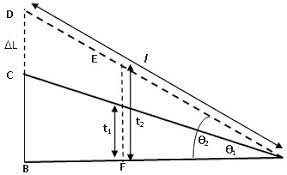
\includegraphics[width=0.8\columnwidth]{images/f3.jpeg}
    \caption{Change in wedge angle with temperature increase}
    \label{fig:3}
\end{figure}

Let $l$ be the length of the top glass plate. Since $\Delta \theta$ is small,
we can see from $\Delta$ACB in Fig (\ref{fig:3}) that,

\begin{align}
    \Delta L = l \Delta \theta
\end{align}

Once we have found out $\Delta L$, we can find $\alpha$ using,

\begin{align}
    \alpha = \frac{l}{L_{RT}} \left(\frac{\Delta L}{\Delta T}\right)
\end{align}

Using Eq. (8) we have,

\begin{align}
    \alpha = \frac{l}{L_{RT}} \left(\frac{\Delta \theta}{\Delta T}\right)
\end{align}

where, $L_{RT}$ is the length of the metal plate at room temperature. Also, $\Delta \theta/\Delta T$ is given by the slope of $\theta$ vs $T$ plot. Hence, we can find out $\alpha$.

Typical values of $\alpha$ for aluminium, copper and brass at room
temperature are 23.1 $\times$ 10$^{-6}$ K$^{-1}$, 16.6 $\times$ 10$^{-6}$ K$^{-1}$ and 20.3
$\times$ 10$^{-6}$ K$^{-1}$ respectively.

\section{Experimental Setup}

\subsection*{Apparatus}

\begin{enumerate}
    \item Two Glass plates
    \item Fizeau's interferometer
    \item Thermocouple and temperature indicator
    \item Travelling Microscope
    \item Variable transformer
    \item Sodium vapour lamp
    \item Brass rod
    \item Heater\\
\end{enumerate}

The schematic design of the experimental set up is shown in Fig. (\ref{fig:1}). It consists of an
interferometer assembly along with a travelling microscope attached. The sample is usually a small metal rod --- brass in this case --- which is sorrounded by a heater, which is a small cement tube over
which a heating element is wound. A thermocouple is inserted such that it is
close to the sample. As the metal expands, the support rod on top of the metal will move up, essentially
creating a wedge between the two glass plates.